\documentclass[10pt]{beamer}

\usepackage{fontspec}
\usepackage{xunicode}
\usepackage{xltxtra}
\setsansfont{FreeSans}
\setmonofont{DejaVuSansMono}

\usepackage{listings}
\usepackage{textpos}
\usepackage{tikz}
\usepackage{minted}

\setbeamertemplate{footline}[frame]
\setbeamertemplate{items}[default]
\usetheme{Warsaw}
\usecolortheme{seahorse}
\setbeamertemplate{itemize items}[default]
\setbeamertemplate{navigation symbols}{}
\setbeamertemplate{footline}[frame number]
\lstset{columns=fixed}
\setbeamerfont*{block body}{series=\tt}
\definecolor{lightgray}{rgb}{0.9,0.9,0.9}
\definecolor{midgray}{rgb}{0.5,0.5,0.5}

\usetikzlibrary{arrows,positioning,fit,backgrounds}
\tikzset{
    %Define standard arrow tip
    >=stealth',
    %Define style for boxes
    punkt/.style={
           rectangle,
           rounded corners,
           draw=black, very thick,
           text width=6.5em,
           minimum height=2em,
           text centered},
    % Define arrow style
    pil/.style={
           ->,
           thick,
           shorten <=2pt,
           shorten >=2pt,}
}

\newcommand{\light}[1]{\textcolor{gray}{\footnotesize{#1}}}
\newcommand{\code}[4]{\inputminted[linenos, frame=none, firstline=#2, lastline=#3,
  framesep=10pt, bgcolor=lightgray]{#4}{#1}}

\title[Bayecho]{Echo + баесовская кластеризация}
\author{Дмитрий Грошев, Ирина Горбунова\\
  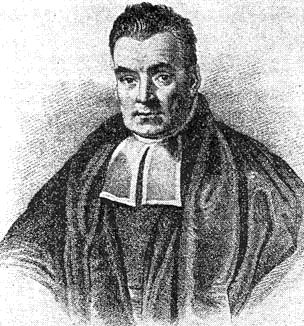
\includegraphics[height=3cm]{thomas_bayes.png}}
\date{04.06.2012}
\institute{СПбАУ}

\begin{document}
\renewcommand*{\inserttotalframenumber}{\pageref{lastframe}}
\begin{frame}
\titlepage
\end{frame}

%% Intro

\begin{frame}
  \begin{center}
    \Large
    Краткое содержание предыдущих серий
  \end{center}
\end{frame}

\begin{frame}{ECHO}
  \begin{itemize}
  \item http://uc-echo.sourceforge.net/
  \item эффективно исправляет ошибки
  \end{itemize}
\end{frame}

\begin{frame}{BayesHammer}
  \begin{itemize}
  \item улучшенная версия утилиты hammer
  \item кластеризует k-меры перед исправлением ошибок
  \item эффективнее начальной версии
  \end{itemize}
\end{frame}

\begin{frame}{Bayecho}
  \begin{itemize}
  \item попытка улучшить ECHO
  \item кластеризация похожих ридов
  \end{itemize}
\end{frame}

%% Echo

\begin{frame}
  \begin{center}
    \Large
    Как работает ECHO
  \end{center}
\end{frame}

\begin{frame}{2 стадии}
  \begin{itemize}
  \item поиск пересекающихся ридов (соседей)
  \item исправление ошибок
  \end{itemize}
\end{frame}

\begin{frame}{ECHO}
  \begin{tikzpicture}[every label/.style={gray},node distance=0.15cm,
                      dummy/.style={minimum width=27mm}]
    \node (dummy1) [dummy] [] {};
    \node (dummy2) [dummy] [right=of dummy1] {};
    \node (dummy3) [dummy] [right=of dummy2] {};
    \node (dummy4) [dummy] [right=of dummy3] {};
    \node (read) [punkt] [below=of dummy1]
          {чтение};
    \node (prefind) [punkt] [below=of dummy2]
          {грубый поиск соседей по хешу k-мера}
          edge [<-] (read);
    \node (fit) [punkt] [below=of prefind,yshift=-5mm]
          {фиттинг $\omega$ и $\epsilon$}
          edge [<-] (prefind);
    \node (find) [punkt] [below=of fit,yshift=-5mm]
          {поиск соседей по $\omega$ и $\epsilon$}
          edge [<-] (fit);
    \node (vote) [punkt] [below=of dummy3]
          {MAP + исправление}
          edge [<-,in=30,out=205] (find);
    \node (reest) [punkt] [below=of vote,yshift=-5mm]
          {пересчёт confusion matrix}
          edge [->,bend left,out=45,in=135] (vote)
          edge [<-,bend right,out=315,in=225] node [right] {EM} (vote);
    \node (output) [punkt] [below=of dummy4]
          {вывод}
          edge [<-,bend left,out=0,in=180] (vote);
    \begin{pgfonlayer}{background}
      \node[fill=black!10,fit=(prefind) (fit) (find),
      label=above:поиск соседей,rounded corners] {};
    \end{pgfonlayer}
    \begin{pgfonlayer}{background}
      \node[fill=black!10,fit=(vote) (reest),
      label=above:исправление,rounded corners] {};
    \end{pgfonlayer}
  \end{tikzpicture}
\end{frame}

\begin{frame}{Поиск соседей}
  \begin{itemize}
  \item поиск точно совпадающего k-мера hashmap'ом
  \end{itemize}
  \begin{center}
    \Large
    $K=max(\frac{L}{5}, \log(\sqrt[4]{N * L}))$
  \end{center}
  \begin{itemize}
  \item подбор $\omega$ и $\epsilon$ (покрытие конкретного нуклеотида должно иметь распределение Пуассона)
  \item поиск неточных соседей по $\omega$ и $\epsilon$
  \end{itemize}
\end{frame}

\begin{frame}{Исправление}
  \begin{itemize}
  \item В группе соседей делается MAP по каждому нуклеотиду и confusion matrix
  \item На основе исправленных ридов пересчитывается confusion matrix
  \item Повторять до схождения
  \end{itemize}
  Это EM-алгоритм
\end{frame}

\begin{frame}{MAP}
  \begin{center}
    \Large
    Maximum A Posteriori
    \[P(A_i) = \prod_{j=1}^{N} \Phi_{READS_{j,i}, A}\]
    \[\operatorname*{arg\,max}_{X=A,T,G,C} P(X)\]
  \end{center}
\end{frame}

%% Our work

\begin{frame}
  \begin{center}
    \Large
    Что сделали мы
  \end{center}
\end{frame}

\begin{frame}
    \begin{tikzpicture}[every label/.style={gray},node distance=0.15cm,
                      dummy/.style={minimum width=27mm}]
    \node (dummy1) [dummy] [] {};
    \node (dummy2) [dummy] [right=of dummy1] {};
    \node (dummy3) [dummy] [right=of dummy2] {};
    \node (dummy4) [dummy] [right=of dummy3] {};
    \node (read) [punkt] [below=of dummy1]
          {чтение};
    \node (prefind) [punkt] [below=of dummy2]
          {грубый поиск соседей по хешу k-мера}
          edge [<-] (read);
    \node (fit) [punkt] [below=of prefind,yshift=-5mm]
          {фиттинг $\omega$ и $\epsilon$}
          edge [<-] (prefind);
    \node (find) [punkt] [below=of fit,yshift=-5mm]
          {поиск соседей по $\omega$ и $\epsilon$}
          edge [<-] (fit);
    \node (clust) [punkt] [below=of dummy3,style={draw=red}]
          {K-Means++}
          edge [<-,in=30,out=199] (find);
    \node (vote) [punkt] [below=of clust,yshift=-5mm]
          {MAP + исправление}
          edge [<-] (clust);
    \node (reest) [punkt] [below=of vote,yshift=-5mm]
          {пересчёт confusion matrix}
          edge [->,bend right,out=290,in=250] node [right] {EM} (clust)
          edge [<-] (vote);
    \node (output) [punkt] [below=of dummy4]
          {вывод}
          edge [<-,bend left,out=90,in=180] (vote);
    \begin{pgfonlayer}{background}
      \node[fill=black!10,fit=(prefind) (fit) (find),
      label=above:поиск соседей,rounded corners] {};
    \end{pgfonlayer}
    \begin{pgfonlayer}{background}
      \node[fill=black!10,fit=(clust) (vote) (reest),
      label=above:исправление,rounded corners] {};
    \end{pgfonlayer}
  \end{tikzpicture}
\end{frame}

\begin{frame}{K-Means}
  \begin{itemize}
  \item выбираются произвольные центры
  \item для каждой точки ищется ближайший центр (диаграма Вороного)
  \item пересчитываются центры
  \end{itemize}
  Это тоже EM
\end{frame}

\begin{frame}{K-Means}
  \begin{center}
    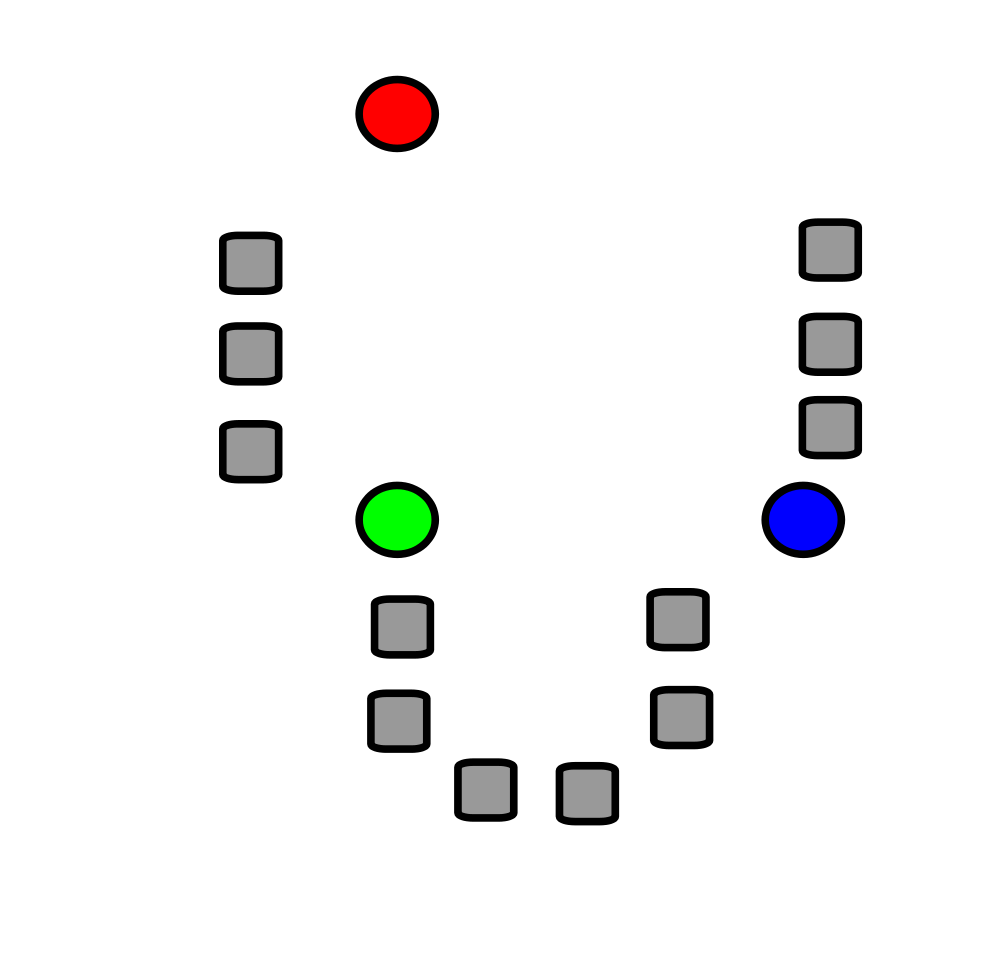
\includegraphics[height=8cm]{clustering1.png}
  \end{center}
\end{frame}

\begin{frame}{K-Means}
  \begin{center}
    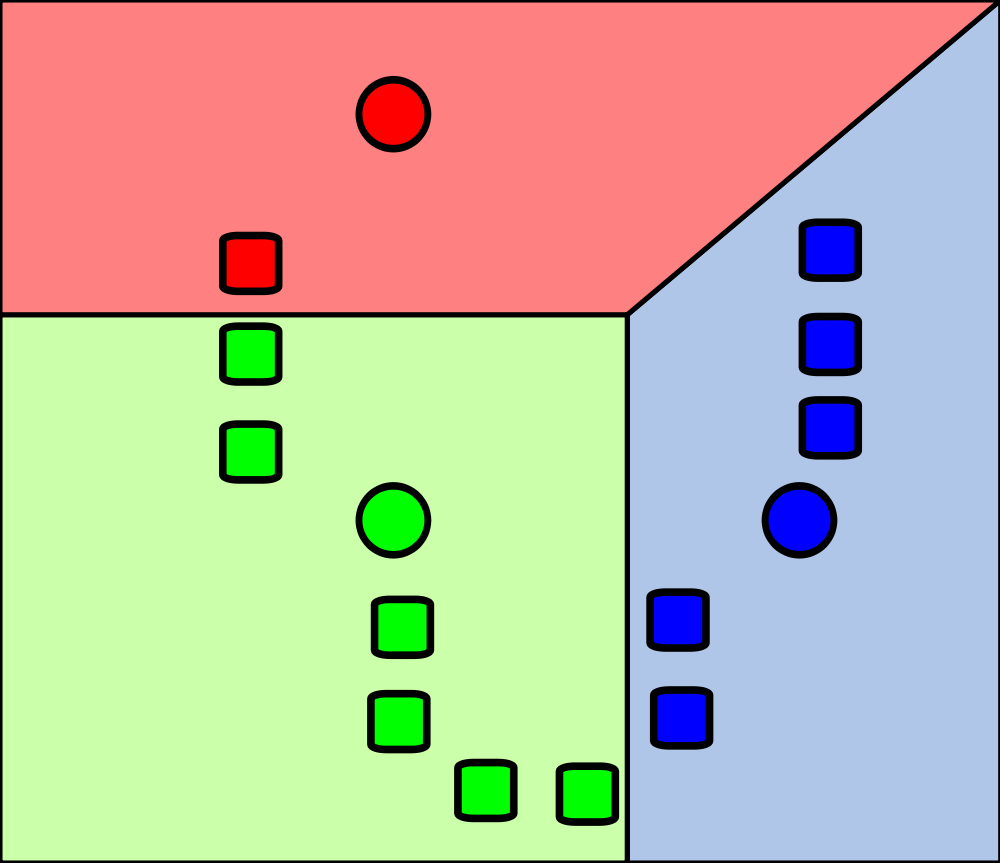
\includegraphics[height=8cm]{clustering2.png}
  \end{center}
\end{frame}

\begin{frame}{K-Means}
  \begin{center}
    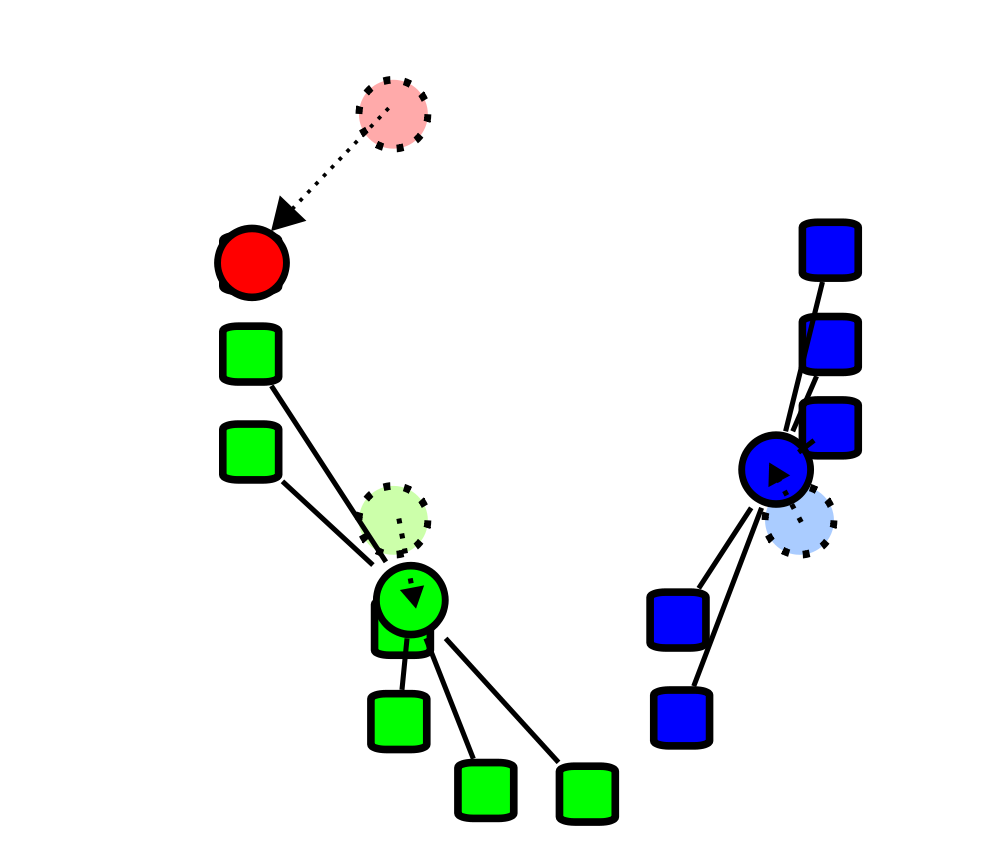
\includegraphics[height=8cm]{clustering3.png}
  \end{center}
\end{frame}

\begin{frame}{K-Means}
  \begin{center}
    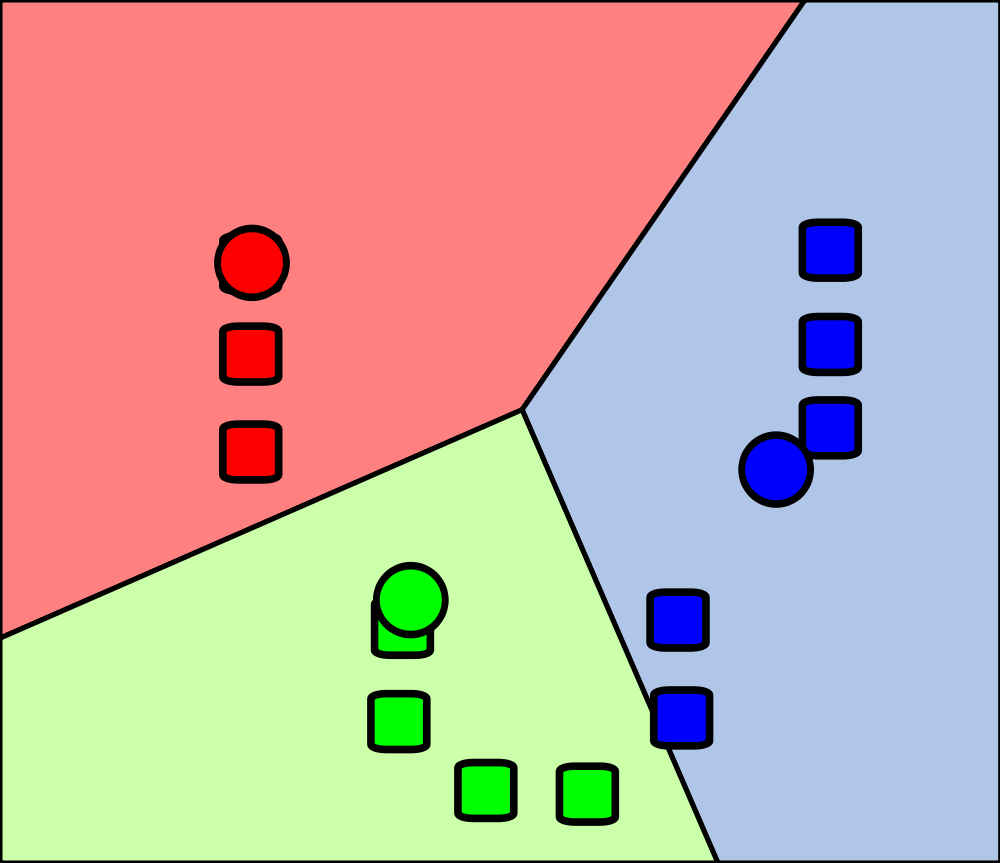
\includegraphics[height=8cm]{clustering4.png}
  \end{center}
\end{frame}

\begin{frame}{K-Means++}
  Модификация K-Means с более сложной инициализацией
  \begin{itemize}
  \item центроидом выбирается случайная точка
  \item подсчитывается расстояние от каждой точки до ближайшего центроида
  \item новый центроид выбирается из оставшихся точек с вероятностью, пропорциональной квадрату расстояния от остальных центроидов
  \end{itemize}
\end{frame}

\begin{frame}[fragile]{Проблема}
  Риды не полностью совпадают (в отличие от k-меров):
\begin{verbatim}
 ATGCATGCA
   TCATGTACGG
  TGCATGCAC
\end{verbatim}
\end{frame}

\begin{frame}[fragile]{Решение}
  Добавим спецсимвол:
\begin{verbatim}
 ATGCATGCA___
 __TCATGTACGG
 _TGCATGCAC__
\end{verbatim}
  Расстояние от \_ до любого символа = 0.
\end{frame}

\begin{frame}{Инициализация}
  Если выбран неполный центроид, дополнить из ближайших (случайный нуклеотид пропорционально расстоянию)
\end{frame}

\begin{frame}[fragile]{Инициализация}
\begin{verbatim}
 ___ATGC
 GCGCTGC
 GCGCTAC
 GCGCT__  <---
 TATATAT
 TCTAT__
 TATGTAT
\end{verbatim}
\end{frame}

\begin{frame}[fragile]{Инициализация}
\begin{verbatim}
 ___ATGC
 GCGCTGC  *
 GCGCTAC  *
 GCGCT__  <---
 TATATAT
 TCTAT__
 TATGTAT
\end{verbatim}
\end{frame}

\begin{frame}[fragile]{Инициализация}
\begin{verbatim}
 ___ATGC
 GCGCTGC
 GCGCTAC
[GCGCTGC] <---
 TATATAT
 TCTAT__
 TATGTAT
\end{verbatim}
\end{frame}

\begin{frame}{Поиск ближайшего центроида}
  Расстояние = 1 - likelihood
\end{frame}

\begin{frame}[fragile]{Поиск новых центроидов}
  Снова MAP:
\begin{verbatim}
group1    group2
___ATGC   TATATAT
GCGCTGC   TCTAT__
GCGCTAC   TATGTAT
GCGCT__
-------   -------
GCGCTGC   TATATAT
\end{verbatim}
\end{frame}

\begin{frame}{Результаты}
  \begin{itemize}
  \item кластеризация кластеризует
  \item запускается
  \item на больших наборах данных ещё не запускали
  \end{itemize}
\end{frame}

\begin{frame}\label{lastframe}
  \begin{center}
    \Large
    Вопросы?
  \end{center}
\end{frame}
